\documentclass[a4paper,12pt]{scrreprt}
\usepackage[T1]{fontenc}
\usepackage[utf8]{inputenc}
\usepackage[ngerman]{babel}
\usepackage[table]{xcolor}% http://ctan.org/pkg/xcolor
%\usepackage{\textit{graphicx\textit{\textit{}}}} <- ??
\usepackage{graphicx}
\usepackage{tabu}



\begin{document}


\author{Dominik Backhausen\and Daniel Dimitrijevic\and Alexander Rieppel\and Thomas Traxler}
\title{Projektantrag\\ LAN Yourself}
\date{10.09.2013}
\maketitle

\section*{Ausgangssituation}
Bestehende VPN Lösungen und Software für den Low-know-how Bereich sind zwar funktional und existent, jedoch sehr oft in der Praxis schlicht unzufriedenstellend. Oft wegen benutzerunfreundlichem oder unübersichtlicher Benutzeroberfläche bzw. eingeschränkter Funktionalität. Darüber hinaus basieren besagte Lösungen meist ausschließlich auf einer Server-Client Architektur. Deshalb soll aus diesem Projekt eine, auf einer existenten VPN-Lösung basierende, Software hervorgehen, welche eine benutzerfreundliche Oberfläche und möglichst viele Funktionen vereint. Dabei ist zu beachten, dass diese Lösung komplett ohne Server auskommt, d.h. nach Peer-to-Peer Prinzip funktioniert. Dabei sind die Peers in Netzwerken organisiert und über sowohl Unicast- als auch Multicast-Adressen ansprechbar.



\section*{Ziele}

	Im Rahmen des Projektes soll eine leicht bedienbare Software entwickelt werden, die den Aufbau eines virtuellen lokalen Netzwerkes sicherstellt. Wichtig ist dabei, dass diese Software nicht auf einer Server-Client Architektur basiert, sondern mit Hilfe einer Peer-to-Peer Lösung realisiert wird. Dabei ist zu beachten, dass es kein Ziel ist diese Lösung selbst zu entwickeln sondern lediglich die Software, eine zugehörige Benutzeroberfläche und die Funktionalitäten die auf eine bestehende Lösung aufgesetzt werden.
	
	Zu den wichtigsten Punkten gehören gute Kompatibilität und Performance die grundsätzlich zu jeder Zeit von der Software gewährleistet werden muss. Um dies sicherzustellen, können Programmprofile angelegt werden, in denen bestimmte Optionen im Verhalten der Software, im Umgang mit bestimmten Programmen definiert und gespeichert werden können. Da die Software auch für Benutzer mit wenig Know-How gedacht ist, wird sehr viel wert auf eine intuitive aber möglichst dezente Benutzeroberfläche wertgelegt. 
	
	\subsection*{Kann-Ziele}
	\begin{itemize}
	\item Optimierung des Datendurchsatzes
	\item Single- oder Multinode Interaktion mit anderen Netzwerken
	\item Mögliche Einstellungen zur Optimierung des Datenverkehrs durch User
	\item Onion-Routing über bestimmte Netzwerkteilnehmer zur Anonymisierung
	\item Freigabe der Internetverbindung im Netzwerk
	\end{itemize}	
		
	\section*{Projektbeschreibung}
		
		Aus dem Projekt soll eine Software hervorgehen die, auf einer bestehenden Lösung basierend, eine VPN-Verbindung mit Hilfe von Peer-to-Peer Technologie aufbaut. Die Software ist prinzipiell für Benutzer gedacht die über wenig Know-How verfügen und soll ohne weitere Einstellungen funktionieren. Das Programm muss dazu lediglich gestartet werden. Allerdings wird es, speziell für erfahrenere Benutzer, Optionen geben, die den Funktionsumfang wesentlich erweitern z.B. Internetfreigabe, Portweiterleitung, etc. 
			
	\section*{Kritische Erfolgsfaktoren}
		Ein Problem könnte fehlende Funktionalität bei der bestehenden VPN-Lösung darstellen, da wir uns beim Verbindungsaufbau und der konkreten Netzwerkfunktionalität, komplett auf die bestehende Lösung verlassen müssen. Einfachheit und Bedienbarkeit sind zwar ein Anliegen hoher Priorität, allerdings kann trotzdem nicht ausgeschlossen werden, dass die Benutzeroberfläche schlicht an diesem scheitert. Darüber hinaus ist es möglich, manche Funktionen nicht in vollem Umfang, aufgrund von technischen Problemen, implementieren zu können.
	\section*{Termine}
	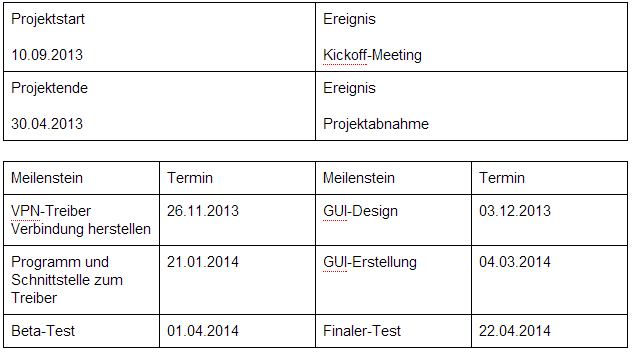
\includegraphics{./Termine}

	
	\section*{Projektorganisation}
	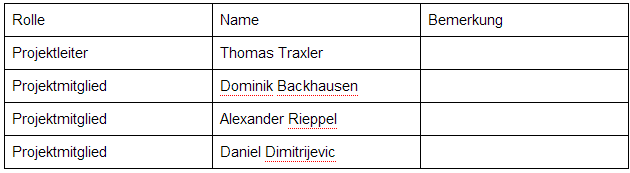
\includegraphics{./Projektorganisation}
		
\end{document}